\begin{problem}{Mostrando grafos}{Standard input}{Standard output}{1 second}{}

% Original idea         
% Problem statement     
% Testset               

Dado un \'arbol $ T = (V, E)$ como un conjunto de v\'ertices $V = \lbrace 1, 2, \dots, n \rbrace$, y un conjunto de aristas $E = \lbrace (p, q) / p, q \in V \rbrace$ con la condici\'on de que existe un nodo ra\'iz $r \in V$, y que hay $n-1$ aristas. Por conveniencia, se considerar\'a un grafo dirigido, y para cada elemento $(p, q) \in E$, indicar\'a que existe arista desde $p$ hacia $q$. Por ejemplo, la siguiente figura muestra un \'arbol de con 12 nodos. 

\begin{figure}[h]
\centering
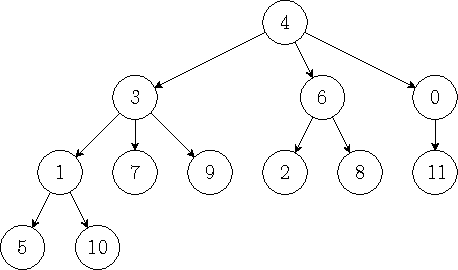
\includegraphics[width=8cm]{images/tree.pdf}
\end{figure}

Tu deber es recorrer el grafo y mostrarlo por niveles, es decir, primero la raiz (nodo 4), luego sus hijos (nodos 3, 6, y 0), luego los hijos de estos nodos q se encuentran en el siguiente nivel (nodos 1, 7, 9, 2, 8, y 4), y as\'i sucesivamente. Para el ejemplo de la figura anterior, la respuesta que se busca ser\'ia la siguiente:

\begin{verbatim}
      4
      3 6 0
      1 7 9 2 8 11
      5 10
\end{verbatim}

\InputFile
El problema contiene varios casos de prueba. La primera l\'inea es un entero $T$ $(1\leq T \leq 10^2)$ que denota el número de casos de prueba. Cada caso está compuesto por dos l\'ineas, en la primera de ellas se encuentra el n\'umero entero $N$ indicando la cantidad de nodos que tend\'ra el grafo ($1 \leq N \leq 10^3$). Luego, en la segunda l\'inea del caso de prueba se encuentran $N-1$ pares de n\'umeros $p, q$ ($0 \leq p, q < n$, $p \neq q$) que representan las aristas del \'arbol en cuesti\'on. El nodo ra\'iz es determinado como aquel nodo que no tiene aristas entrantes, m\`as s\'i aristas salientes.

\OutputFile
Para cada caso de prueba, el programa deber\'a imprimir ``\texttt{Caso \#i:}'' (sin comillas) y a partir de la siguiente linea el grafo por niveles. 

\Example

\begin{example}
\exmp{%%INPUT
3
2
0 1
5
0 1 1 2 2 3 3 4
11
4 3 3 1 6 2 0 11 3 9 4 0 1 5 6 8 1 10 3 7 4 6%%END-INPUT
}{ %%OUTPUT
Caso \#1:
0
1
Caso \#2:
0
1
2
3
4
Caso \#3:
4
3 6 0
1 7 9 2 8 11
5 10
} %%END-OUTPUT
\end{example}

\end{problem}
